\begin{center}
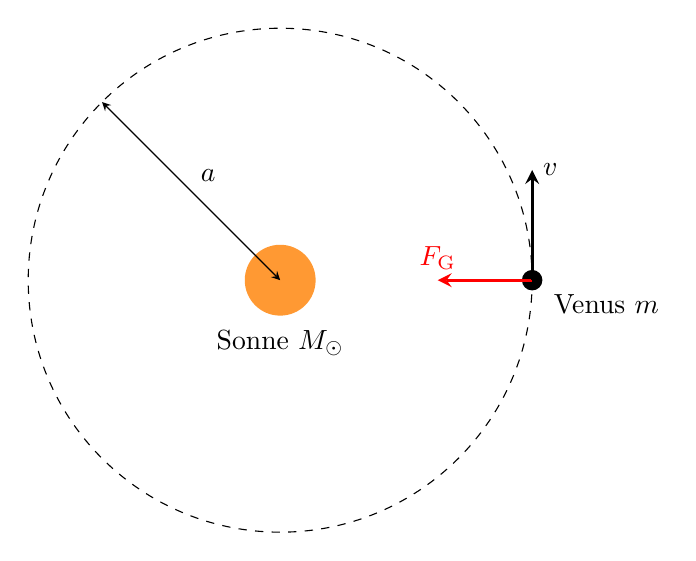
\begin{tikzpicture}[>=stealth]
 \draw[dashed] (0,0) circle (3.2);
 \fill[orange!80] (0,0) circle (0.45);
 \node at (0,-0.8) {Sonne $M_\odot$};
 \draw[<->] (0,0) -- (-2.263,2.263) node[midway, above right] {$a$};
 \fill (3.2,0) circle (0.13);
 \node[anchor=west] at (3.35,-0.3) {Venus $m$};
 \draw[->, very thick, red] (3.2,0) -- (2.0,0) node[above] {$F_\mathrm{G}$};
 \draw[->, very thick] (3.2,0) -- (3.2,1.4) node[right] {$v$};
\end{tikzpicture}
\end{center}

Die Venusbahn ist fast ein Kreis (numerische Exzentrizität \exVO). Die Gravitationskraft der Sonne ist die Zentripetalkraft der Kreisbewegung mit Radius $a$ und Umlaufzeit $T$:
\begin{align}
 G\,\frac{M_\odot\, m}{a^2} &= m\,\frac{4\pi^2 a}{T^2}
\end{align}
Die Planetentabelle (FoTaBe S.~212) gibt für die Venus $a = \aVO$ und $T = \TVO$. Damit ist
\begin{align}
 M_\odot &= \MSbF \\
   &= \frac{4\pi^2\cdot\left(\aV\right)^3}{\ncG\cdot\left(\TV\right)^2} \\
   &= \MSb \approx \result{\MSbS{3}}
\end{align}
Die Formelsammlung (FoTaBe S.~211) gibt $M_\odot = \MSo$. Die relative Abweichung
\begin{align}
 \frac{M_\odot-M_\text{Tab}}{M_\text{Tab}} &= \abw
\end{align}
ist kleiner als die Unsicherheit der Gravitationskonstante (vier Stellen); die Werte stimmen überein. (Die Masse der Venus ist gegenüber der Sonnenmasse vernachlässigbar.)
